\chapter{Use-Case Analysis}

\section{Actor Overview}

\begin{table}[H]
\centering
\caption{Implemented actors}
\begin{tabularx}{\textwidth}{L{0.23\textwidth}Y}
\toprule
\textbf{Actor} & \textbf{Role in the system} \\
\midrule
Admin & Privileged internal user who can manage merchants, internal users, credentials, and merchant portal users. \\
Ops & Day-to-day internal operations user who can inspect operational evidence and execute allowed lifecycle and recovery workflows. \\
Merchant backend & Merchant-owned server application that calls payment and refund APIs using HMAC credentials. \\
Merchant portal user & Human merchant user who logs into Merchant Dashboard using merchant id, email, and password. \\
Provider simulator & Simulated external provider that sends payment and refund result callbacks. \\
Scheduler/worker trigger & External trigger that invokes implemented expiration and due-webhook delivery services. \\
\bottomrule
\end{tabularx}
\end{table}

\section{Core Gateway Use Cases}

\begin{longtable}{L{0.11\textwidth}L{0.24\textwidth}L{0.19\textwidth}L{0.36\textwidth}}
\caption{Core implemented use cases}\\
\toprule
\textbf{ID} & \textbf{Use case} & \textbf{Primary actor} & \textbf{Result} \\
\midrule
\endfirsthead
\toprule
\textbf{ID} & \textbf{Use case} & \textbf{Primary actor} & \textbf{Result} \\
\midrule
\endhead
UC001 & Onboard and activate merchant & Admin/Ops & Merchant profile, onboarding case, credential, activation status, and audit trail are created. \\
UC002 & Create dynamic QR payment & Merchant backend & A pending payment and QR payload are created or an identical pending payment is reused. \\
UC003 & Process payment result callback & Provider simulator & Callback evidence is stored; the pending payment becomes success or failed, or reconciliation evidence is created. \\
UC004 & Create full refund and process result & Merchant backend and provider simulator & A full refund is created and later finalized from provider evidence. \\
UC005 & Deliver webhook with retry and manual recovery & Scheduler/worker trigger, Admin/Ops & Webhook attempts are persisted, retries are scheduled, and failed events can be recovered manually. \\
\bottomrule
\end{longtable}

\section{Dashboard Use Cases}

\begin{longtable}{L{0.12\textwidth}L{0.28\textwidth}L{0.20\textwidth}L{0.30\textwidth}}
\caption{Implemented dashboard use cases}\\
\toprule
\textbf{ID} & \textbf{Use case} & \textbf{Actor} & \textbf{Implemented behavior} \\
\midrule
\endfirsthead
\toprule
\textbf{ID} & \textbf{Use case} & \textbf{Actor} & \textbf{Implemented behavior} \\
\midrule
\endhead
DUC001 & Login and view operations overview & Admin/Ops & Internal users authenticate and inspect operational metrics. \\
DUC002 & Manage merchant lifecycle & Admin/Ops & Users create merchants, inspect onboarding and credentials, and apply allowed lifecycle actions. \\
DUC003 & Provision merchant portal users & Admin & Admin creates, updates, deactivates or reactivates, and resets merchant portal users. \\
DUC004 & Inspect operational evidence & Admin/Ops & Users inspect payments, refunds, webhooks, reconciliation, and audit logs. \\
DUC005 & Login and change password & Merchant portal user & Merchant users authenticate with a portal session and can change their own password. \\
DUC006 & View overview and analytics & Merchant portal user & Users view scoped summary metrics and 7, 30, or 90 day analytics. \\
DUC007 & Explore payments, refunds, and webhooks & Merchant portal user & Users browse and inspect records owned by their merchant only. \\
DUC008 & View profile and credentials & Merchant portal user & Users read merchant profile and credential metadata without raw secrets. \\
\bottomrule
\end{longtable}

\section{Use-Case Diagram}

\begin{figure}[H]
\centering
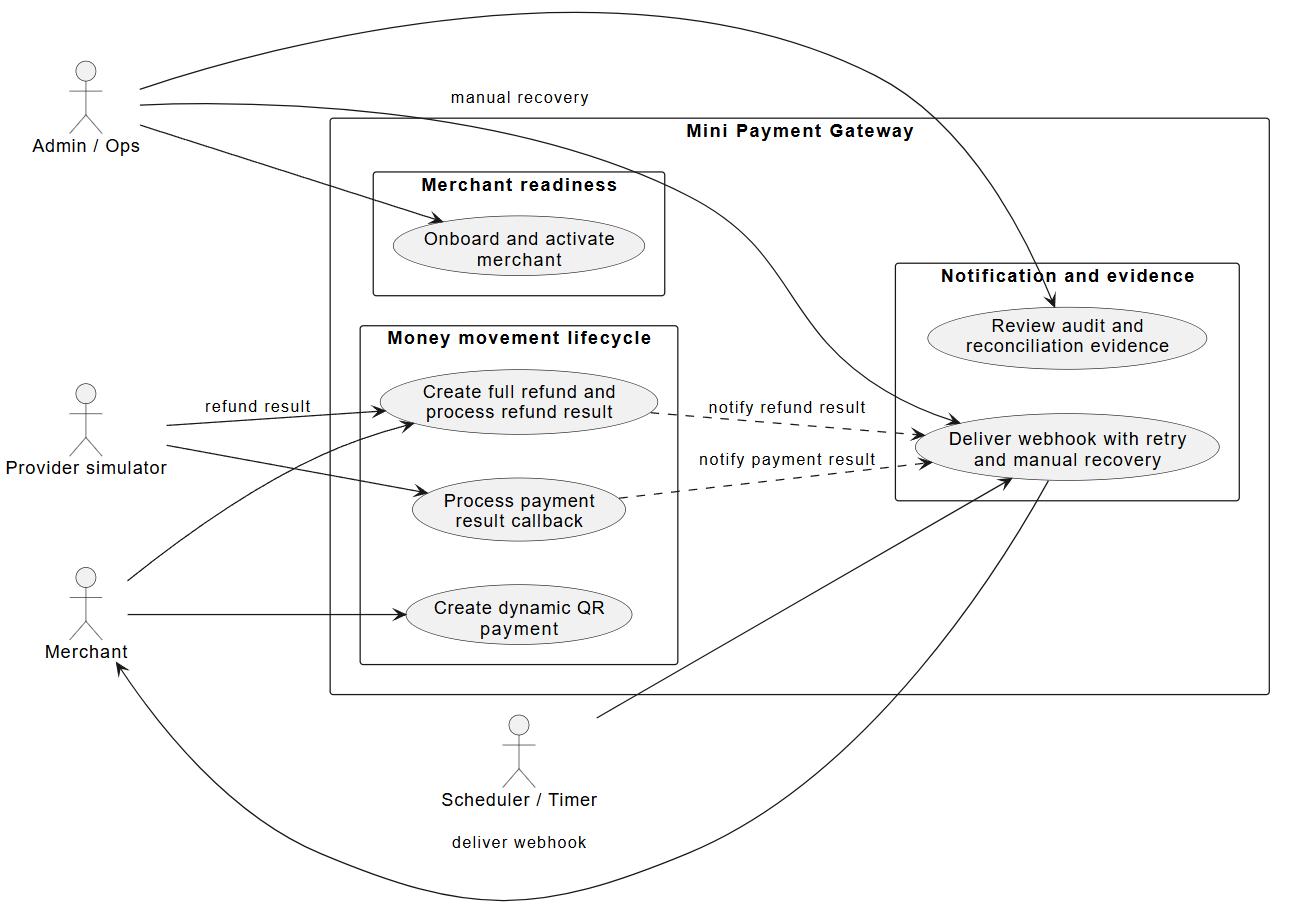
\includegraphics[width=\linewidth]{figures/general-usecase.png}
\caption{Implemented use-case overview. Operational dashboard use cases are
separated from merchant money-flow use cases.}
\end{figure}
